
\section{Training Settings}
\label{sec:training_details}
Table~\ref{tab:llm_arch_adamw} summarizes the model architecture and the optimizer parameters of \olmo-7B as well as recent similar-sized models. 


\begin{table*}[t]
    \centering
    \small
    \begin{tabular}{l|lllll}
        \toprule
        & \textbf{\olmo-7B} & \textbf{LLaMA2-7B} & \textbf{OpenLM-7B} & \textbf{Falcon-7B} & \textbf{PaLM-8B} \\
        \hline
       Dimension & 4096 & 4096 & 4096 & 4544 & 4096 \\
        Num heads & 32 & 32 & 32 & 71 & 16 \\
        Num layers & 32 & 32 & 32 & 32 & 32 \\
        MLP ratio & $\sim$8/3 & $\sim$8/3 & $\sim$8/3 & 4 & 4 \\
        Layer norm type & non-parametric & RMSNorm & parametric & parametric & parametric \\
        Positional embeddings & RoPE & RoPE & RoPE & RoPE & RoPE \\
        Attention variant & full & GQA & full & MQA & MQA \\
        Biases & none & none & in LN only & in LN only & none \\
        Block type & sequential & sequential & sequential & parallel & parallel \\
        Activation & SwiGLU & SwiGLU & SwiGLU & GeLU & SwiGLU \\
        Sequence length & 2048 & 4096 & 2048 & 2048 & 2048 \\
        Batch size (instances) & 2160 & 1024 & 2048 & 2304 & 512 \\
        Batch size (tokens) & $\sim$4M & $\sim$4M & $\sim$4M & $\sim$4M & $\sim$1M \\
        Weight tying & no & no & no & no & yes \\
        \hline
        Warmup steps & 5000 & 2000 & 2000 & 1000 \\
        Peak LR & \texttt{3.0E-04} & \texttt{3.0E-04} & \texttt{3.0E-04} & \texttt{6.0E-04} \\
        Minimum LR & \texttt{3.0E-05} & \texttt{3.0E-05} & \texttt{3.0E-05} & \texttt{1.2E-05} \\
        Weight decay & 0.1 & 0.1 & 0.1 & 0.1 \\
        Beta1 & 0.9 & 0.9 & 0.9 & 0.99 \\
        Beta2 & 0.95 & 0.95 & 0.95 & 0.999 \\
        Epsilon & \texttt{1.0E-05} & \texttt{1.0E-05} & \texttt{1.0E-05} & \texttt{1.0E-05} \\
        LR schedule & linear & cosine & cosine & cosine \\
        Gradient clipping & global 1.0 & global 1.0 & global 1.0 & global 1.0 \\
        Gradient reduce dtype & FP32 & FP32 & FP32 & BF16 \\
        Optimizer state dtype & FP32 & most likely FP32 & FP32 & FP32 \\
        \bottomrule
    \end{tabular}
    % \vspace{1em}
    \caption{LM architecture and optimizer comparison at the 7--8B scale. In the ``layer norm type" row, ``parametric" and ``non-parametric" refer to the usual layer norm implementation with and without adaptive gain and bias, respectively. All models are trained using AdamW.}
    \label{tab:llm_arch_adamw}
\end{table*}





\section{Power Consumption and Carbon Footprint}
\label{sec:carbon}

Following previous literature \citep{strubell-etal-2019-energy, patterson2021carbon, wu2022sustainable, dodge2022measuring}, we estimate the total energy consumed and carbon released while pretraining our models by calculating the total power consumption required for training, and then multiplying it by the carbon emission intensity of the power grid where the model was trained. While reporting these operational emissions is standard practice, it does not account for other sources of emissions such as the embodied emissions due to the manufacturing, transportation, and disposal of hardware and datacenter infrastructure, lifetime operational emissions due to use, rebound effects, or other environmental impacts such as water consumption or mining. Thus our estimates should be viewed as lower bounds.

We calculate the total power consumption for our models by measuring the power consumption of a single node every 25ms, calculating an average across the entire training run, and multiplying by the total number of nodes. We then account for the energy efficiency of the data center by multiplying the previous total by a power usage effectiveness (PUE) factor, which we set to 1.1, representing a conservative 10\% energy consumption overhead typical of energy efficient datacenters.\footnote{\protect\url{https://www.nrel.gov/computational-science/measuring-efficiency-pue.html}}\footnote{\protect\url{https://www.google.com/about/datacenters/efficiency/}} We estimate that pretraining our 7B models consumed \textbf{239 MWh} of energy.

To calculate carbon emissions, we multiply the total power consumption by a carbon intensity factor, measured in kg CO$_2$ emitted per KWh, based on the physical location of the data center where each model was trained. The model trained on A100-40GB GPUs was trained in Australia, so we assume a carbon intensity factor of 0.610, the national average for Australia in 2022.\footnote{\protect\url{https://www.cleanenergyregulator.gov.au/Infohub/Markets/Pages/qcmr/december-quarter-2022/Emissions-Reduction.aspx}} The model trained on MI250X GPUs was trained in the LUMI supercomputer, which runs on 100\% renewable, carbon-neutral energy, so we assume a carbon intensity factor of 0. LUMI is powered entirely by hydroelectric power and some sources \citep{Ubierna2022} measure the carbon intensity factor of hydroelectric power to be 0.024, which would imply total carbon emissions of 3.54 tCO$_2$eq.{\footnote{\url{https://www.lumi-supercomputer.eu}}} However, we rely on the official LUMI data for our calculations, and thus we estimate total pretraining emissions of \textbf{69.78 tCO$_2$eq}.\footnote{These metrics were in part collected using Carbonara's AI agent and monitoring platform. Learn more at: \url{https://trycarbonara.com}} In Table \ref{tab:co2-emissions} we compare our models with other previously released models based on publicly available information.
% In Table \ref{tab:co2-emissions} we compare our models with other previously released models based on publicly available information. \nascomment{info in the rest of this paragraph seems redundant with table + caption.  remove?} \jacobm[]{good q -- I'll defer to jesse and emma. I'm okay with keeping or removing} Gopher-280B \citep{rae2022scaling} reports a PUE of 1.08, a carbon intensity factor of 0.330, and a total emissions of 380 tCO$_2$eq. BLOOM-176B reports a PUE of 1.2, a carbon intensity factor of 0.057, and a total power consumption from GPUs of 433 MWh, resulting in 29.64 tCO$_2$eq \citep{luccioni2022estimating}. OPT-175B \citep{zhang2022opt} and LLaMA \citep{touvron2023llama1, touvron2023llama2} models assume a PUE of 1.1, an average power consumption per GPU of 400W (the maximum power draw for an A100-80GB), and a carbon intensity of 0.231 and 0.385, respectively, leading to 82.24 tCO$_2$eq emitted for OPT-175B, 13.86 tCO$_2$eq for LLaMA 7B, and 31.22 tCO$_2$eq for LLaMA 2 7B. T5-11B \citep{raffel2023exploring} reports a PUE of 1.12, a carbon intensity factor of 0.545, a total power consumption of 85.7 MWh, and a total emissions of 46.7 tCO$_2$eq \citep{patterson2021carbon}.

% In Table \ref{tab:co2-emissions} we compare our models with other previously released models. In addition to power consumption from GPUs and the carbon intensity of the local grid, each reports a PUE for the data center used during training: Gopher-280B \citep{rae2022scaling} reports a PUE of 1.08, BLOOM-176B \citep{workshop2022bloom, luccioni2022estimating} reports a PUE of 1.2, OPT-175B \citep{zhang2022opt} and LLaMA \citep{touvron2023llama1, touvron2023llama2} models assume a PUE of 1.1, and T5-11B \citep{raffel2023exploring, patterson2021carbon} reports a PUE of 1.12. OPT-175B and LLaMA models also assume an average power consumption per GPU of 400W (the maximum power draw for an A100-80GB).

We hope that openly releasing our models can reduce future emissions by allowing others to avoid the need to pretrain models from scratch, and give insights into the true cost of developing state of the art models. We also highlight that our estimates are lower bounds, because they do not include other critical pieces of development such as debugging, hyperparameter tuning, and downtime.

\begin{table*}
\begin{tabular}{l|cccccc}
\toprule
 & GPU Type & \begin{tabular}[c]{@{}c@{}}GPU Power\\ Consumption\\(MWh)\end{tabular} & \begin{tabular}[c]{@{}c@{}}Power\\ Usage\\ Effectiveness\end{tabular} & \begin{tabular}[c]{@{}c@{}}Carbon\\ Intensity\\ (kg CO$_2$e/KWh)\end{tabular} & \begin{tabular}[c]{@{}c@{}}Carbon\\ Emissions\\ (tCO$_2$eq)\end{tabular} \\ \hline
\textbf{Gopher-280B} & TPU v3 & 1,066 & 1.08 & 0.330 & 380 \\
\textbf{BLOOM-176B} & A100-80GB & 433 & 1.2 & 0.057 & 30 \\
\textbf{OPT-175B} & A100-80GB & 324 & 1.1 & 0.231 & 82 \\
\textbf{T5-11B} & TPU v3 & 77 & 1.12 & 0.545 & 47 \\
\textbf{LLaMA-7B} & A100-80GB & 33 & 1.1 & 0.385 & 14 \\
\textbf{LLaMA2-7B} & A100-80GB & 74 & 1.1 & 0.385 & 31 \\
% \hline % Changed to color highlight to be consistent with Table 6. Feel free to change back.
\rowcolor{olmocolor}
[\dimexpr\tabcolsep+0.1pt\relax] 
\textbf{OLMo-7B} & MI250X & 135 & 1.1 & 0.000* & 0* \\
\hline  % Without the line there is a weird white pixel issue here. Coloring the line also looks strange.
\rowcolor{olmocolor}
[\dimexpr\tabcolsep+0.1pt\relax]
\textbf{OLMo-7B} & A100-40GB & 104 & 1.1 & 0.610 & 70 \\
\arrayrulecolor{black}\bottomrule
\end{tabular}
% \vspace{1em}
\caption{CO$_2$ emissions during pretraining. We estimate the total carbon emissions for various models using publicly available data on PUE, carbon intensity of local power grid, and reported power consumption. Numbers for Gopher-280B \citep{rae2022scaling}, BLOOM-176B \citep{luccioni2022estimating}, OPT-175B \citep{zhang2022opt}, T5-11B \citep{patterson2021carbon}, LLaMA \citep{touvron2023llama1}, and LLaMA2 \citep{touvron2023llama2} are taken from their respective papers. See Section \ref{sec:carbon} for details on how tCO2eq was calculated.\\
% We take a carbon intensity set to Australia's national average of 0.610 kg CO$_2$e per KWh \escomment{Note to also change Australia here; alternatively, description in this caption (and *) is a bit redundant with the section; might just refer to section for more details for everything that currently follows the ``See Section 3.6".} for our model trained on A100-40GB GPUs, and to 0.0 for our model trained on MI250X GPUs in the LUMI supercomputer because it runs on ``100\% renewable, carbon-neutral energy"\addtocounter{footnote}{-1}\protect\footnotemark.\\
\addtocounter{footnote}{-1}* LUMI runs entirely on hydroelectric power\protect\footnotemark and some estimates \citep{Ubierna2022} measure the intensity factor of hydroelectric power to be 0.024, implying total emissions of 3.54 tCO$_2$eq.}
\label{tab:co2-emissions}
\end{table*}





\section{Additional Evaluation}
\label{sec:add_eval}

\begin{figure*}[t]
    \centering
    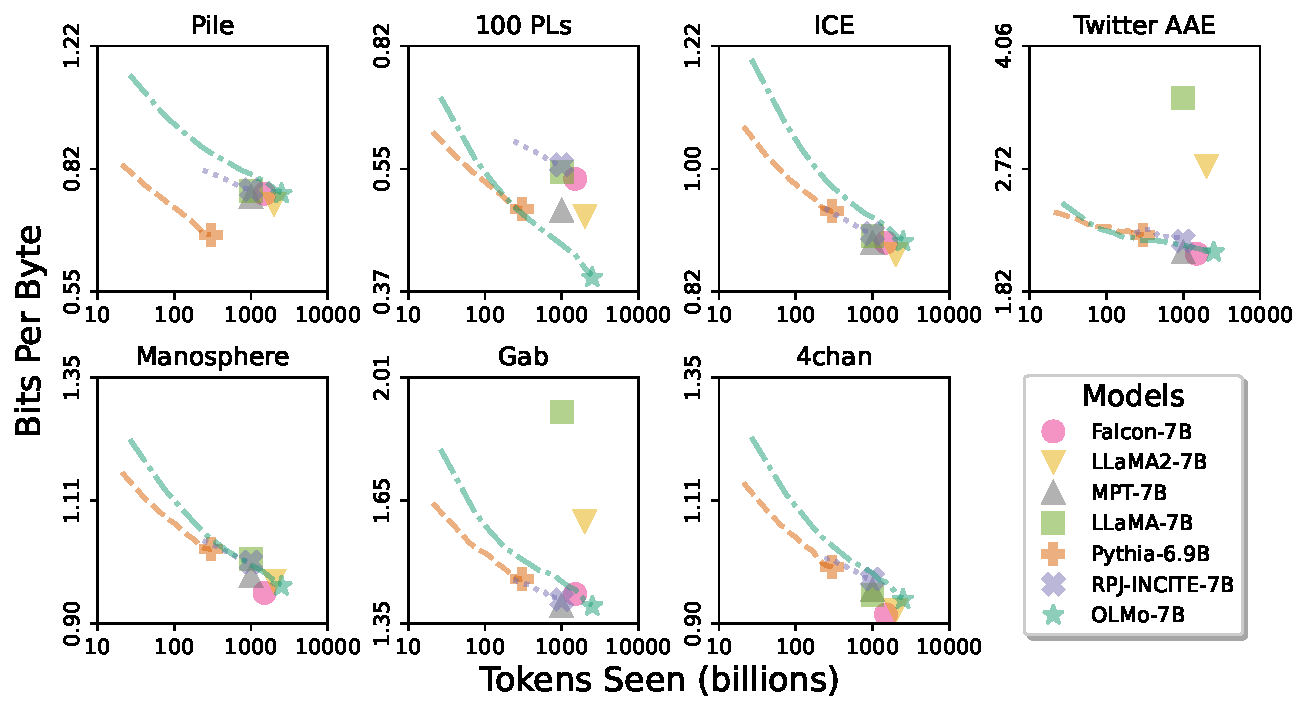
\includegraphics[width=\textwidth]{figures/paloma_bpb_over_tokens_seen_per_source_not_clean.pdf}
    \caption{Bits per byte for each of the 7 remaining Paloma data sources not aggregated in Figure~\ref{fig:paloma_bpb_over_tokens_seen_per_source_clean}.
    }
    \label{fig:paloma_bpb_over_tokens_seen_per_source_not_clean}
\end{figure*}

\paragraph{Additional perplexity results} In Figure~\ref{fig:paloma_bpb_over_tokens_seen_per_source_not_clean} we provide results for each of the 7 data sources in Paloma \citep{magnusson2023paloma} that are excluded from the combined metric in Figure~\ref{fig:paloma_bpb_over_tokens_seen_per_source_clean}. Some of these sources such as Pile \citep{gao2020pile} and ICE \citep{GREENBAUM_1996} are not publicly available at this time. Dolma 100 Programming Languages \citep{dolma} consists of code data that is not supported by the decontamination approach used in Paloma. TwitterAAE \citep{blodgett-etal-2016-demographic}, along with ICE, are datasets for targeted analyses of disparities in performance between different dialects and as such should be evaluated separately. And finally, the Manosphere, Gab, and 4chan corpora \citep{Horta_Ribeiro_2021, zannettougab, papasavva_2020} are intended to examine model fit to language from fringe online communities that are studied for prevalent hate speech and toxicity. Thus minimizing perplexity on these fringe corpora is not always desirable.

One notable result here is that \model is much farther ahead of the other models on Dolma 100 Programming Languages (100 PLs). Note that this effect may be due in part to underestimation from contamination, as decontaminating code data is beyond the scope of the method in Paloma. At the same time other models that are trained on code data from GitHub such as RPJ-INCITE-7B, that are just as likely to have contamination, fair much worse. Another factor then is that \model trains on code data with exactly the same post-processing as that in 100 PLs while the code data in other models will have been processed differently. Similarly, Pile evaluation demonstrates these in-distribution and potential contamination effects as Pythia-6.9B achieves top performance despite being trained on almost an order of magnitude fewer tokens than \model.

The results on the remaining 5 targeted sources should be interpreted with care, as Paloma often finds that perplexity on these sources is dominated by superficial features such as low average document length rather than fit to that which would actually be salient to members of these speech communities. TwitterAAE and Gab have among the shortest documents in Paloma contributing to unusually high bits per byte in this figure. Other than these two, the models are notably very closely grouped in a data scaling trend in ICE, Manosphere, and 4chan.

\paragraph{Additional end-task results} Next, in Table~\ref{table:additional-end-task}, we provide results from zero-shot evaluation of \model on 6 additional end-tasks apart from the 8 in our core evaluation suite. These tasks are \texttt{headqa\_en}~\citep{head-qa}, \texttt{logiqa}~\citep{logi-qa}, \texttt{mrpc}~\citep{mrpc}, \texttt{qnli}~\citep{glue}, \texttt{wic}~\citep{wic}, and \texttt{wnli}~\citep{glue}. 





\begin{table*}[!t]
\centering 
% \adjustbox{max width=\columnwidth}{
\begin{tabular}{@{}c|cccccc|c
% |>{\columncolor[HTML]{C0C0C0}}c @{}
}
\toprule
% \cellcolor[HTML]{C0C0C0}model/end-task
& headqa\_en & logiqa & mrpc & qnli & wic & wnli & avg. \\
\hline
\textbf{Falcon-7B}     & 38.6 & 23.7 & 62.8 & 49.8 & 49.5 & 47.9 & 45.4 \\
\textbf{LLaMA-7B}      & 38.7 & 19.5 & 68.6 & 50.1 & 49.1 & 52.1 & 46.4 \\
\textbf{LLaMA2-7B}     & 39.5 & 26.1 & 69.1 & 49.4 & 49.8 & 45.1 & 46.5 \\
\textbf{MPT-7B}        & 37.4 & 22.9 & 67.7 & 52.1 & 48.1 & 47.9 & 46.0 \\
\textbf{Pythia-6.9B}   & 40.1 & 21.5 & 65.4 & 53.8 & 55.0 & 38.0 & 45.6 \\
\textbf{RPJ-INCITE-7B} & 36.9 & 27.8 & 58.8 & 53.8 & 48.9 & 57.8 & 47.3 \\
% \hline
\rowcolor{olmocolor}
[\dimexpr\tabcolsep+0.1pt\relax]
\textbf{OLMo-7B}       & 37.3 & 23.4 & 68.4 & 49.1 & 50.2 & 56.3 & 47.5 \\
% [\dimexpr\tabcolsep+0.1pt\relax]
\bottomrule
\end{tabular}
% }
% \vspace{1em}
\caption{Zero-shot evaluation of \model on 6 additional end-tasks apart from the 8 present in our core evaluation suite. Once again, we compare \model to 6 other model checkpoints which are publicly available. We find that \model outperforms the other models on aggregate taken over 6 additional end-tasks from this table, however these tasks were also found to provide limited signal during training (see Figure~\ref{fig:additional-task-acc-progression}).}
\label{table:additional-end-task}
\end{table*}

We note, however, that in contrast to our core evaluation set described in Section~\ref{sec:downstream_evaluation}, we found these additional end-tasks to have less stable performance during model development, and to provide a limited signal.  This is illustrated in Figure~\ref{fig:additional-task-acc-progression}, where we see the progress of task performance throughout training to be more random (compare with the more stable upward trends in Figure~\ref{fig:core-tasks-progression}). While tasks such as \texttt{mrpc} and \texttt{wic} appear more stable, they offered additional difficulties related to performance being tied to random chance (e.g., \texttt{wic}) or the tendency of models to make spurious predictions (e.g., always predicting a single label) that either inflate or deflate performance due to dataset class imbalances (e.g., \texttt{mrpc}). We therefore caution against relying too heavily on these tasks when measuring model performance throughout training and comparing models. 


\begin{figure*}[!t]
\centering
\makebox[\columnwidth][c]{
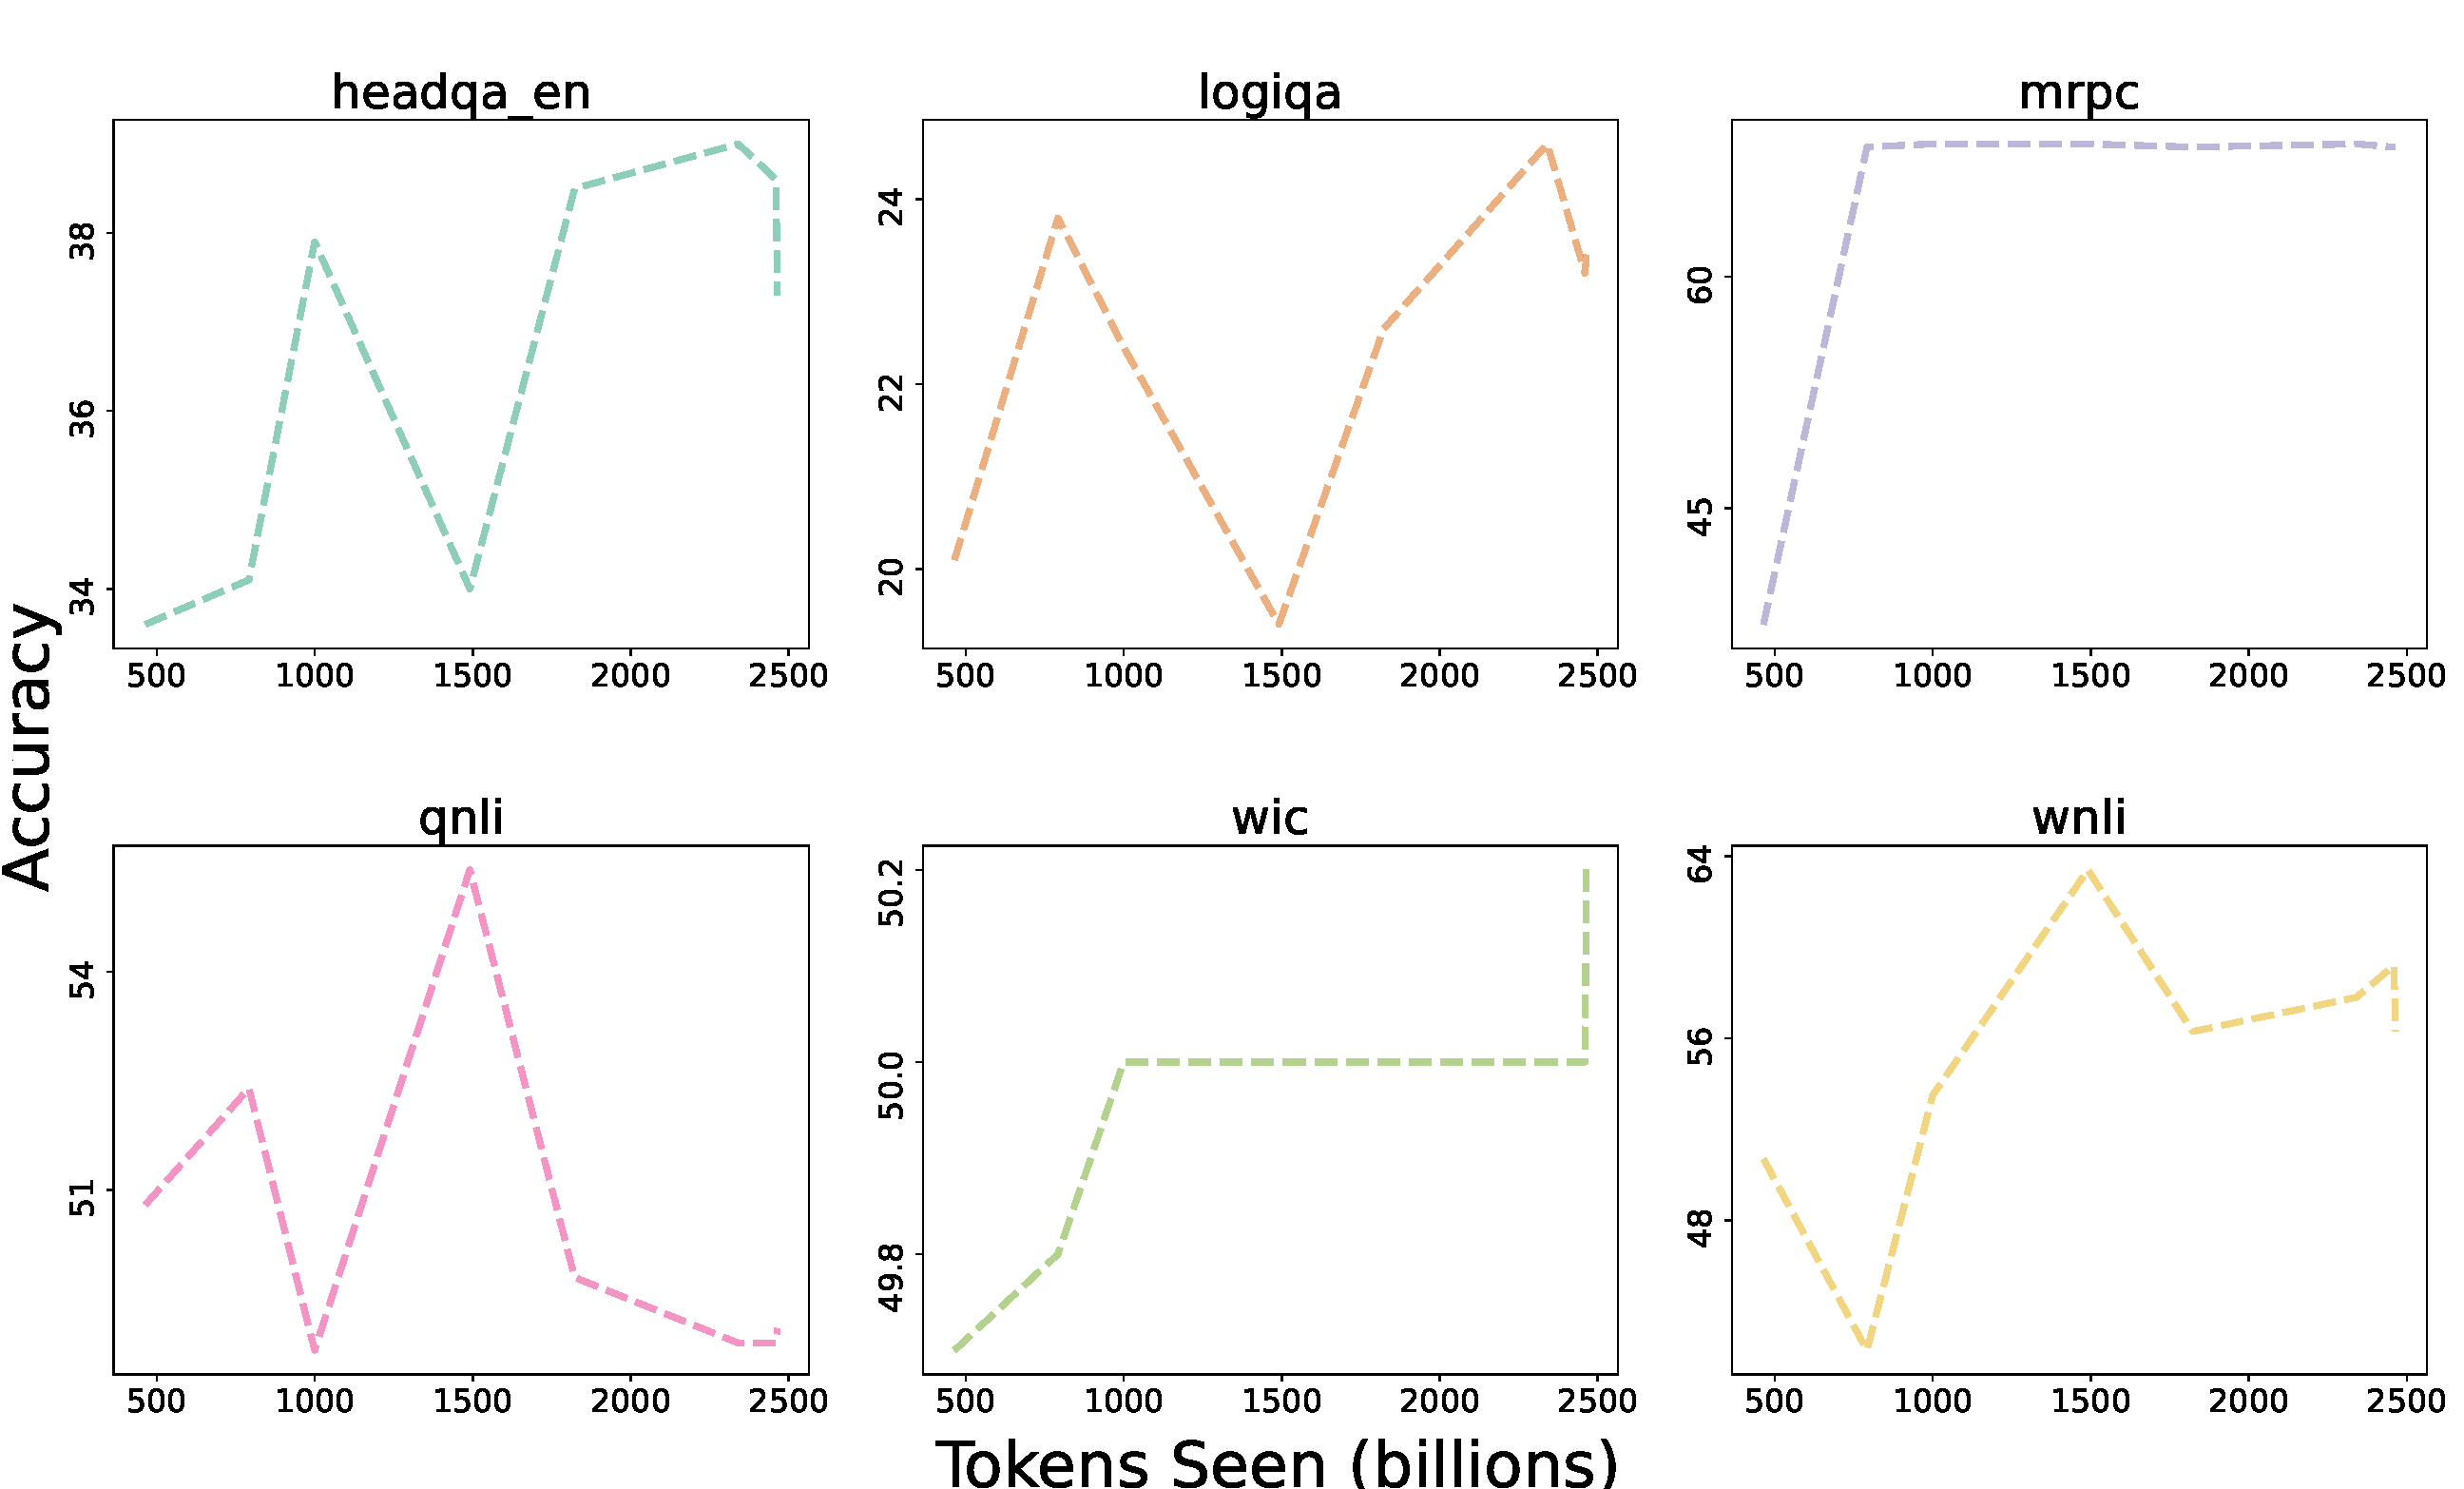
\includegraphics[width=\textwidth]{figures/additional_tasks.pdf}
}
\caption{Accuracy score progression of \model on 6 additional end-tasks. The performance of these additional end-tasks was unstable and provided limited signal during model development.}
\label{fig:additional-task-acc-progression}
\end{figure*}

\section{Adaptation Training Details}
\label{app:adaptation_training_details}
We use the following hyperparameters when instruction tuning \olmo. These were chosen through small pilot experiments.

\begin{itemize}
\setlength{\itemsep}{0pt}
    \item Learning rate: $2 \times 10^{-6}$
    \item Epochs: 3
    \item Warmup: Linear warmup for the first 3\% of total training time, and then linear cooldown to a learning rate of 0 over the remaining steps.
    \item Weight decay: 0
    \item Gradient clipping: 0
    \item Maximum sequence length: 2048
    \item Data: \tulu V2 SFT mix, resplit such that long conversations are split into 2048-token chunks and replacing the hardcoded split with data about \olmo. Data is publically available.\footnote{\url{https://huggingface.co/datasets/allenai/tulu-v2-sft-mixture-olmo-2048}}
\end{itemize}

After instruction finetuning, we then use the following hyperparameters for DPO training, following \citet{ivison2023camels}:

\begin{itemize}
\setlength{\itemsep}{0pt}
    \item Learning rate: $5 \times 10^{-7}$
    \item $\beta$: 0.1
    \item Epochs: 3
    \item Warmup: Linear warmup for the first 10\% of total training time, and then linear cooldown to a learning rate of 0 over the remaining steps.
    \item Weight decay: 0
    \item Gradient clipping: 0
    \item Maximum sequence length: 2048
    \item Data: A modified form of UltraFeedback~\citep{cui2023ultrafeedback}, with TruthfulQA prompts removed. We used the `fixed' variant released by Argilla, which uses the average of GPT-generated aspect-based scores to determine chosen and rejected pairs.\footnote{\url{https://huggingface.co/datasets/argilla/ultrafeedback-binarized-preferences-cleaned}}
\end{itemize}


\section{Adaptation Evaluation and Model details}
\label{app:adaptation-evals-description}
We choose the models in Table~\ref{table:results-adaptation} by choosing the `canonical' best versions (that is, the best instruction-tuned or otherwise adapted models released by the same organisation) of the base models we compare against in Table~\ref{table:results-end-task}. We additionally compare to \tulu 2 to show the current best models trained using the \tulu mix used to finetune \olmo. We display evaluations on MMLU, AlpacaEval, ToxiGen, and Truthfulness to focus on displaying how instruction tuning can generally help capabilities (MMLU), how the models perform in an open-ended chat setting (AlpacaEval), and to test how instruction tuning aids in model safety and truthfulness (AlpacaEval, ToxiGen). We additionally report \olmo's performance over the entire \tulu evaluation suite in Table~\ref{table:results-adaptation-full}.


\begin{table*}[t]
\adjustbox{max width=2\columnwidth}{
\begin{tabular}{@{}l|cccccccc
% |>{\columncolor[HTML]{C0C0C0}}c @{}
}
\toprule
% \cellcolor[HTML]{C0C0C0}\textbf{model/end-task}
\textbf{Model} & \textbf{MMLU}   & \textbf{GSM8k}      & \textbf{BBH}        & \textbf{TydiQA} & \textbf{Codex-Eval} & \textbf{AlpacaEval} & \textbf{ToxiGen} & \textbf{TruthfulQA} \\
& \textbf{0-shot} & \textbf{8-shot CoT} & \textbf{3-shot CoT} & \textbf{1-shot} & \textbf{Pass@10}    & \textbf{\%win}       & \textbf{\% Toxic} & \textbf{\% Info + True}  \\
\hline
\textbf{\model}        & 28.3 & 8.5 & 31.7 & 32.3 & 21.4 & - & 81.4 & 31.6 \\
\textbf{+SFT}        & 47.3 & 15.5 & 36.9 & 35.2 & 28.6 & 57.0 & 14.4 & 41.2 \\
\textbf{+SFT+DPO}        & 46.1 & 11.0 & 35.8 & 21.7 & 27.8 & 69.3  & 1.7 & 52.0 \\
\bottomrule
\end{tabular}
}
\vspace{1em}
\caption{Evaluation of \model models before and after instruction finetuning and DPO training on the full \tulu evaluation suite. Lower is better for ToxiGen and higher is better for other metrics.}
\label{table:results-adaptation-full}
\end{table*}

We provide a brief description of each model evaluated in Table~\ref{table:results-adaptation} below. For all models, we use the provided chat template for prompt formatting when available. 
\begin{itemize}[leftmargin=*]
    \item MPT Chat: A version of MPT 7B finetuned on the ShareGPT-Vicuna~\citep{vicuna2023}, HC3~\citep{guo-etal-2023-hc3}, Alpaca~\citep{alpaca}, HH-RLHF~\citep{bai2022training}, and Evol-Instruct~\citep{xu2024wizardlm} datasets. Retrieved from \url{https://huggingface.co/mosaicml/mpt-7b-chat}.
    \item Falcon Instruct: A version of Falcon 7B finetuned on the Baize~\citep{xu2023baize}, GPT4All~\citep{gpt4all}, GPTeacher~\citep{gpteacher}, and Refined-Web English~\citep{penedo2023therd} datasets. Retrieved from \url{https://huggingface.co/tiiuae/falcon-7b-instruct}.
    \item RPJ-INCITE Chat: A version of RPJ-INCITE 7B finetuned on the OASST1~\citep{kopf2023openassistant} and Dolly V2~\citep{DatabricksBlog2023DollyV2} datasets. Retrieved from \url{https://huggingface.co/togethercomputer/RedPajama-INCITE-7B-Chat}.
    \item Llama-2 Chat: A version of Llama 2 7B finetuned on a mixture of instruction datasets and further trained with RLHF. We refer the reader to \citet{touvron2023llama2} for further details.
    \item \tulu 2: A version of Llama 2 7B finetuned on a mixture of instruction datasets (the \tulu 2 mix). We refer the reader to \citet{ivison2023camels} for further details.
    \item \tulu 2+DPO: \tulu 2 further trained with DPO on the UltraFeedback dataset~\citep{cui2023ultrafeedback}. We refer the reader to \citet{ivison2023camels} for further details.
    \item OLMo+SFT: A version of \olmo 7B fintuned on the same data as \tulu 2.
    \item OLMo+SFT+DPO: OLMo+SFT further trained with DPO on the UltraFeedback dataset~\citep{cui2023ultrafeedback}.
\end{itemize}

We additionally provide a brief description of each evaluation setting from Table~\ref{table:results-adaptation}:
\begin{itemize}[leftmargin=*]
    \item \textbf{MMLU}: We use the official MMLU~\citep{hendryckstest2021} evaluation script and prompts available at \url{https://github.com/hendrycks/test}, with modifications to allow for batch processing. We evaluate using 0 few-shot examples, following the original setup of MMLU. We report average accuracy across test examples.
    \item \textbf{ToxiGen}: We follow the setup in \citet{touvron2023llama2}, but use the original set of prompts from \citet{hartvigsen2022toxigen}, which are designed to elicit toxic generations for certain groups. We take only the prompts designed to produce toxic language (`hateful' prompts) and use 500 prompts per group to reduce evaluation costs. For base language models, we pass in the original ToxiGen prompts unchanged and greedily decode up to the first new line (or a maximum of 512 tokens). For instruction-tuned models, we place the prompt in the corresponding template, and ask the model to complete the prompt, until the model generates a stop token (or a maximum of 512 tokens). We pass the generated text into a roberta-large model trained to detect toxic content finetuned as part of \citet{hartvigsen2022toxigen}.\footnote{\url{https://huggingface.co/tomh/toxigen\_roberta}} We then report the percentage of generations deemed toxic by the classifier.
    \item \textbf{TruthfulQA}: Following \citet{touvron2023llama2}, we mainly use the generation setting of TruthfulQA \citep{lin2022truthfulqa}. The TruthfulQA dataset contains 818 questions, which are used to prompt the tested model to generate answers. We use the default QA prompt format with 6 in-context QA examples. We follow the official script in their official implemention\footnote{\url{https://github.com/sylinrl/TruthfulQA/}} to do greedy decoding and answer postprocessing. We train two LLaMA 2-based classifiers for judging the truthfulness and informativeness of the model response, due to the deprecation of GPT-3 making exact replication of the original TruthfulQA evaluation infeasible. We find that the LLaMA 2 judges are generally able to match the performance of the original GPT-3-based judges used by \citet{lin2022truthfulqa}. We report the rate of the responses being truthful and informative (\% Informative and Truthful) following \citet{touvron2023llama2}. We only report the \% Informative and Truthful as our primary metric.
    \item \textbf{AlpacaEval}: We use the package provided by \citet{alpaca_eval}, following the default setup which asks the evaluated model to generate responses for 805 prompts and employ GPT-4 to compare the response with \instructgpt{003}. We employ the ``alpaca\_eval\_gpt4'' annotator. We allow the evaluated model to generate up to 2048 tokens, without specifying special stop sequences. The reported win-rate is the percentage of model generations that GPT-4 reports as being preferred over the generations from \instructgpt{003}.
\end{itemize}

